\documentclass[12pt, a4paper, oneside]{report}
\usepackage[margin=0.9in, top=0.9in, bottom=0.9in]{geometry}
\usepackage[utf8]{inputenc}
\usepackage[T1]{fontenc}
\usepackage{lmodern}
\usepackage{amsmath, amssymb}
\usepackage{booktabs}
\usepackage{array}
\usepackage{tabularx}
\usepackage{fancyhdr}
\usepackage{float}
\usepackage{graphicx}
\usepackage{xcolor}
\usepackage{enumitem}
\usepackage{titlesec}
\usepackage{hyperref}
\usepackage{tikz}
\usetikzlibrary{arrows.meta, positioning}
\tikzset{
  blk/.style={rectangle, rounded corners=4pt, line width=0.8pt, align=center,
              font=\sffamily\small, inner sep=5pt},
  blueb/.style={blk, draw=blue!70!black, fill=blue!6},
  tealb/.style={blk, draw=teal!70!black, fill=teal!6},
  orangeb/.style={blk, draw=orange!80!black, fill=orange!9},
  redb/.style={blk, draw=red!70!black, fill=red!6},
  greenb/.style={blk, draw=green!50!black, fill=green!7},
  pipe/.style={-{Stealth[length=2.4mm]}, line width=0.8pt, draw=black!80},
  steplbl/.style={font=\sffamily\scriptsize\bfseries, fill=white, draw=black!25,
                  line width=0.4pt, inner sep=2pt, rounded corners=1.5pt},
}

\graphicspath{{figures/}}
\setlist{itemsep=2pt, topsep=4pt}
\setlength{\emergencystretch}{2em}
\sloppy

\titleformat{\chapter}[display]
  {\normalfont\LARGE\bfseries}{\chaptertitlename\ \thechapter}{3pt}{\LARGE}
\titlespacing*{\chapter}{0pt}{-35pt}{10pt}
\titlespacing*{\section}{0pt}{8pt}{4pt}
\titlespacing*{\subsection}{0pt}{6pt}{3pt}

% --- Header and Footer ---
\pagestyle{fancy}
\setlength{\headheight}{14.5pt}
\fancyhf{}
\fancyhead[L]{\small\sffamily UCS503 -- Software Engineering Project}
\fancyhead[R]{\small\sffamily Real-Time Flood Risk AI Prediction System}
\fancyfoot[C]{\thepage}
\renewcommand{\headrulewidth}{0.4pt}
\fancypagestyle{plain}{\fancyhf{}\fancyfoot[C]{\thepage}\renewcommand{\headrulewidth}{0pt}}

% --- Hyperref Setup ---
\hypersetup{
    colorlinks=true,
    linkcolor=blue!70!black,
    citecolor=teal!70!black,
    urlcolor=blue!60!black,
    pdftitle={Real-Time Flood Risk AI Prediction System: Prototype Report},
    pdfauthor={Amit Bishnoi, Diksha Garg},
    pdfsubject={UCS503 Software Engineering Project}
}

\newcommand{\code}[1]{\texttt{#1}}

\begin{document}

% =========================================================================
% TITLE PAGE
% =========================================================================
\begin{titlepage}
    \centering
    \vspace*{0.5cm}

    {\Large\bfseries UCS503 -- Software Engineering Project}\\[0.3cm]
    {\large Academic Year 2026--2027}\\[1.5cm]

    {\Huge\bfseries Real-Time Flood Risk AI Prediction System}\\[0.7cm]
    {\large\textit{A Data Fusion and Machine Learning Pipeline for Dynamic Disaster Threat Mapping}}\\[2.0cm]

    {\large\textbf{Submitted by:}}\\[0.3cm]
    \begin{tabular}{lll}
        \textbf{1024240005} & Amit Bishnoi & \textit{ML, API \& Frontend Lead} \\
        \textbf{1024240015} & Diksha Garg  & \textit{System Architecture \& Data Engineering} \\
    \end{tabular}\\[0.5cm]
    {\normalsize Computer Science and Engineering Department (CSED)}\\[1.2cm]

    {\large\textbf{Submitted to:}}\\[0.2cm]
    {\large\textbf{Dr. Jeelani Asif}}\\[0.1cm]
    {\normalsize Department of Computer Science and Engineering}\\[1.2cm]

    {\normalsize Repository: \url{https://github.com/Flood-Prediction-AI-Team/Flood-Prediction-Using-WeatherAPI-and-historical-thread-mapping}}\\[0.15cm]
    {\normalsize Documentation: \url{https://Flood-Prediction-AI-Team.github.io/Flood-Prediction-Using-WeatherAPI-and-historical-thread-mapping/}}

    \vfill
    {\normalsize\textbf{Prototype Stage Report}}\\[0.15cm]
    {\normalsize\textbf{Computer Science and Engineering Department}}\\[0.1cm]
    {\normalsize Thapar Institute of Engineering and Technology, Patiala}\\[0.4cm]
\end{titlepage}

% =========================================================================
% TABLE OF CONTENTS
% =========================================================================
\pagenumbering{roman}
\tableofcontents
\clearpage
\pagenumbering{arabic}

% =========================================================================
% CHAPTER 1: INTRODUCTION
% =========================================================================
\chapter{Introduction}

\section{Background and Context}

Traditional flood prediction models often rely solely on static geographical contours or standalone historical archives. While modern meteorological APIs provide high-precision real-time atmospheric metrics, they frequently lack historical baseline disaster contexts. Conversely, traditional hazard maps are drawn once and rarely updated, rendering them ineffective during sudden, severe storms. Live weather data and historical disaster records exist in isolated silos, making it difficult for responders to instantly correlate a storm with historical vulnerability.

Before building our complete platform, we evaluated the feasibility of combining REST weather metrics with spatial centroid proximity queries. The proof-of-concept confirmed that fusing asynchronous OpenWeatherMap payloads with historical DFO and EM-DAT disaster records enables accurate, low-latency risk classification.

\subsection{Problem Statement}

Given a target location, we want a system that ingests live meteorological data via external APIs, executes spatial proximity queries against historical flood centroids within a 100km radius, fuses these data streams into feature vectors, and produces a verified threat classification backed by an interactive geospatial dashboard.

\section{Project Objectives}

\begin{enumerate}
    \item Build an automated data ingestion pipeline fetching real-time meteorological metrics via the OpenWeatherMap API with spatial proximity indexing using the Haversine formula.
    \item Engineer a machine learning pipeline (Random Forest classifier) trained on fused historical data and synthetic overlapping datasets to prevent overfitting.
    \item Deploy a responsive frontend dashboard using HTML/CSS, JavaScript, and Leaflet.js to render threat levels and geospatial radius maps in real time.
    \item Implement robust mock weather fallback mechanisms to ensure continuous operation during third-party API rate limits.
    \item Provide comprehensive documentation hosted via MkDocs and GitHub Pages alongside complete unit testing coverage.
\end{enumerate}

\section{Scope of this Prototype}

Following the course roadmap, the prototype stage delivers the full end-to-end pipeline: historical dataset cleaning and merging, Haversine spatial indexing, OpenWeatherMap API integration with fail-safe fallback logic, Random Forest threat classification, and an interactive Leaflet.js frontend dashboard.

% =========================================================================
% CHAPTER 2: METHODOLOGY AND DESIGN
% =========================================================================
\chapter{Methodology and Design}

\section{System Architecture}

\subsection{High-Level Design}

The system is organized as a decoupled 3-tier architecture mapping onto our division of labor: data engineering, machine learning backend, and frontend UI visualization. 

\begin{figure}[H]
\centering
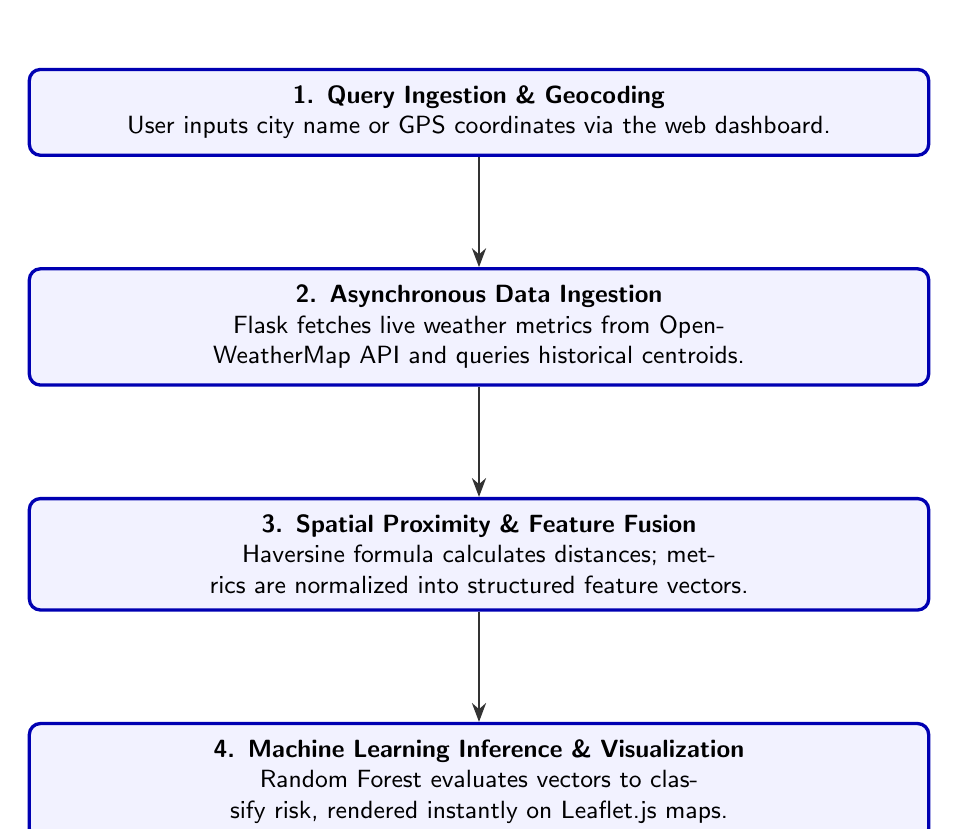
\begin{tikzpicture}[node distance=1.4cm, 
    box/.style={rectangle, rounded corners=4pt, draw=blue!70!black, fill=blue!5, very thick, text width=11cm, align=center, font=\sffamily\small, inner sep=6pt}]
    
    \node[box] (step1) {\textbf{1. Query Ingestion \& Geocoding}\\User inputs city name or GPS coordinates via the web dashboard.};
    \node[box, below=of step1] (step2) {\textbf{2. Asynchronous Data Ingestion}\\Flask fetches live weather metrics from OpenWeatherMap API and queries historical centroids.};
    \node[box, below=of step2] (step3) {\textbf{3. Spatial Proximity \& Feature Fusion}\\Haversine formula calculates distances; metrics are normalized into structured feature vectors.};
    \node[box, below=of step3] (step4) {\textbf{4. Machine Learning Inference \& Visualization}\\Random Forest evaluates vectors to classify risk, rendered instantly on Leaflet.js maps.};

    \draw[pipe] (step1) -- (step2);
    \draw[pipe] (step2) -- (step3);
    \draw[pipe] (step3) -- (step4);
\end{tikzpicture}
\caption{High-Level Data Ingestion and Processing Flow.}
\label{fig:design_flow}
\end{figure}


\section{Machine Learning Strategy and Model Selection}

To reliably evaluate complex, non-linear environmental conditions against historical baselines, selecting the appropriate machine learning architecture is critical. The system relies on a classification paradigm to categorize imminent threat levels.

\subsection{Evaluated Baseline Models}
Prior to finalizing the prediction engine, several algorithmic approaches were considered:
\begin{itemize}
    \item \textbf{Logistic Regression:} Served as the initial linear baseline. While computationally inexpensive, it struggled to capture the complex, non-linear interactions between atmospheric volatility (e.g., rapid humidity spikes) and geographical proximity.
    \item \textbf{Support Vector Machines (SVM):} Effective at drawing decision boundaries in high-dimensional spaces, but computationally heavy and highly sensitive to unscaled environmental outliers during live API fetching.
\end{itemize}

\subsection{Why Random Forest (The Chosen Architecture)?}
The final pipeline utilizes a \textbf{Random Forest Classifier}. It constructs multiple decision trees during training to output a majority-voted class. This ensemble approach was chosen for three distinct advantages:

\begin{enumerate}
    \item \textbf{Noise Robustness:} Averages multiple trees to filter out sudden anomalies and outliers frequently found in live weather API payloads.
    \item \textbf{Non-Linear Fusion:} Seamlessly maps continuous atmospheric metrics (rain, wind) against discrete spatial counts (past regional floods).
    \item \textbf{Interpretability:} Extracts feature importance automatically, allowing the system to verify exactly which metrics triggered a high-risk alert.
\end{enumerate}

\begin{figure}[H]
\centering
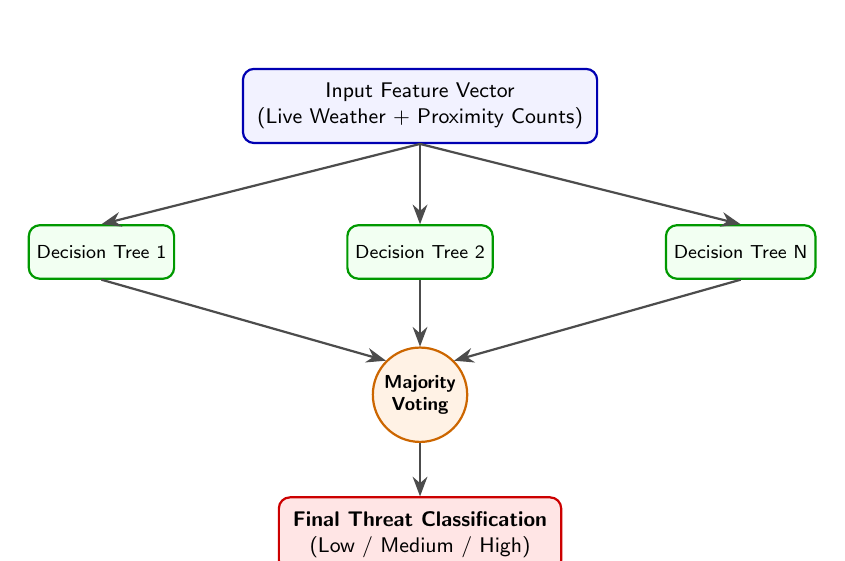
\begin{tikzpicture}[
    scale=0.85, transform shape,
    node distance=1.3cm and 1.8cm,
    box/.style={rectangle, draw=blue!70!black, fill=blue!5, thick, align=center, rounded corners, minimum height=1cm, inner sep=6pt, font=\sffamily\small},
    tree/.style={rectangle, draw=green!60!black, fill=green!5, thick, align=center, rounded corners, minimum height=0.8cm, font=\sffamily\footnotesize},
    vote/.style={circle, draw=orange!80!black, fill=orange!10, thick, align=center, inner sep=2pt, font=\sffamily\footnotesize\bfseries}
]
% Nodes
\node[box] (input) {Input Feature Vector\\(Live Weather + Proximity Counts)};

\node[tree, below left=1.2cm and 1cm of input] (tree1) {Decision Tree 1};
\node[tree, below=1.2cm of input] (tree2) {Decision Tree 2};
\node[tree, below right=1.2cm and 1cm of input] (tree3) {Decision Tree N};

\node[vote, below=1.0cm of tree2] (voting) {Majority\\Voting};
\node[box, fill=red!10, draw=red!80!black, below=0.8cm of voting] (output) {\textbf{Final Threat Classification}\\(Low / Medium / High)};

% Arrows
\draw[-{Stealth[length=2.5mm]}, thick, draw=black!70] (input.south) -- (tree1.north);
\draw[-{Stealth[length=2.5mm]}, thick, draw=black!70] (input.south) -- (tree2.north);
\draw[-{Stealth[length=2.5mm]}, thick, draw=black!70] (input.south) -- (tree3.north);

\draw[-{Stealth[length=2.5mm]}, thick, draw=black!70] (tree1.south) -- (voting.north west);
\draw[-{Stealth[length=2.5mm]}, thick, draw=black!70] (tree2.south) -- (voting.north);
\draw[-{Stealth[length=2.5mm]}, thick, draw=black!70] (tree3.south) -- (voting.north east);

\draw[-{Stealth[length=2.5mm]}, thick, draw=black!70] (voting.south) -- (output.north);

\end{tikzpicture}
\caption{Random Forest Ensemble Architecture for Risk Classification.}
\label{fig:rf_architecture}
\end{figure}

\section{Implementation Details}

\subsection{Data Transformation Pipeline in \code{feature\_engineering.py}}

The core data transformation and preprocessing logic is executed within the \code{feature\_engineering.py} script. Running this module processes raw heterogeneous data streams and outputs a standardized, synchronized feature array ready for model training and live inference.

\begin{itemize}
    \item \textbf{Where the Data Comes From (Input Sources):} 
    The script ingests two primary data origins:
    \begin{enumerate}
        \item \textit{Historical Disaster Archives:} Cleaned CSV records containing global flood epicenters, severity indices, and past occurrence counts stored in \code{Code/Merged\_dataset/fused\_historical\_database.csv}.
        \item \textit{Live Meteorological Payloads:} Real-time atmospheric JSON responses fetched dynamically via the OpenWeatherMap REST API (containing temperature, humidity, wind speed, and precipitation metrics).
    \end{enumerate}
    
    \item \textbf{Data Transformation and Output Generated:} 
    Upon execution, \code{feature\_engineering.py} performs coordinate normalization, calculates geodesic proximity counts within a 100km radius using the Haversine formula, and constructs standardized multi-variable feature vectors. It outputs normalized feature matrices along with serialized feature scalers and encoders.
    
    \item \textbf{Where the Data Goes (Destinations):} 
    The processed feature vectors and normalized arrays are passed directly to the Random Forest training pipeline (\code{train\_model.ipynb}) to serialize model weights into \code{train\_model.pkl}. During live execution, the backend Flask server (\code{backend.py}) invokes these engineered features to evaluate incoming user queries and transmit classified risk levels to the Leaflet frontend dashboard.
\end{itemize}

\subsection{Module 3: Frontend Dashboard and Visualization}

This module renders the user interface (\code{Code/Frontend/}), featuring location search bars, dynamic risk indicator cards, and Leaflet.js map rendering that automatically executes "fly-to" animations and visualizes 50km geospatial threat radius circles. Figure~\ref{fig:frontend_dash} illustrates the deployed prototype interface.

\begin{figure}[H]
    \centering
    % Ensure you upload your frontend screenshot to Overleaf and name it 'frontend_dashboard.png'
    \includegraphics[width=0.95\textwidth, keepaspectratio]{frontend_dashboard.png}
    \caption{Interactive Leaflet.js Frontend Dashboard displaying live weather metrics and assessed threat levels.}
    \label{fig:frontend_dash}
\end{figure}

\end{document}